%\title{LaTeX Portrait Poster Template}
%%%%%%%%%%%%%%%%%%%%%%%%%%%%%%%%%%%%%%%%%
% a0poster Portrait Poster
% LaTeX Template
% Version 1.0 (22/06/13)
%
% The a0poster class was created by:
% Gerlinde Kettl and Matthias Weiser (tex@kettl.de)
% 
% This template has been downloaded from:
% http://www.LaTeXTemplates.com
%
% License:
% CC BY-NC-SA 3.0 (http://creativecommons.org/licenses/by-nc-sa/3.0/)
%
%%%%%%%%%%%%%%%%%%%%%%%%%%%%%%%%%%%%%%%%%

%----------------------------------------------------------------------------------------
%	PACKAGES AND OTHER DOCUMENT CONFIGURATIONS
%----------------------------------------------------------------------------------------

\documentclass[a0,portrait]{a0poster}


\usepackage{geometry}
 \geometry{
a0paper,
 left=20mm,
 right=20mm,
 top=20mm,
 bottom = 20mm
 }


\usepackage{multicol} % This is so we can have multiple columns of text side-by-side
\columnsep=100pt % This is the amount of white space between the columns in the poster
\columnseprule=3pt % This is the thickness of the black line between the columns in the poster

\usepackage[svgnames]{xcolor} % Specify colors by their 'svgnames', for a full list of all colors available see here: http://www.latextemplates.com/svgnames-colors

\usepackage{times} % Use the times font
%\usepackage{palatino} % Uncomment to use the Palatino font

\usepackage{graphicx} % Required for including images
\graphicspath{{figures/}} % Location of the graphics files
\usepackage{booktabs} % Top and bottom rules for table
\usepackage[font=small,labelfont=bf]{caption} % Required for specifying captions to tables and figures
\usepackage{amsfonts, amsmath, amsthm, amssymb} % For math fonts, symbols and environments
\usepackage{wrapfig} % Allows wrapping text around tables and figures
\usepackage[english]{babel}
%\usepackage[utf8x]{inputenc}
\usepackage{colortbl}
\graphicspath {{figures/}}
\usepackage[font=scriptsize,labelfont=bf]{caption}
\usepackage{ragged2e}
\usepackage[T1]{fontenc}
\usepackage{multirow}



\begin{document}

%----------------------------------------------------------------------------------------
%	POSTER HEADER 
%----------------------------------------------------------------------------------------

% The header is divided into two boxes:
% The first is 75% wide and houses the title, subtitle, names, university/organization and contact information
% The second is 25% wide and houses a logo for your university/organization or a photo of you
% The widths of these boxes can be easily edited to accommodate your content as you see fit

\begin{minipage}[b]{0.75\linewidth}
\veryHuge \color{NavyBlue} \textbf{Pedestrian trajectory prediction} \color{Black}\\ % Title
%\vspace{1cm}
\huge \textbf{Rodolphe Farrando \& Romain Gratier}\\[0.5cm] % Author(s)
\huge EPFL -- ENAC Faculty\\[0.4cm] % University/organization
\Large \texttt{\{rodolphe.farrando, romain.gratierdesaint-louis\}@epfl.ch}\\
\end{minipage}
%
\begin{minipage}[b]{0.25\linewidth}

\includegraphics[width=20cm]{./figure/epfl_logo.jpg}\\
\end{minipage}

\vspace{1cm} % A bit of extra whitespace between the header and poster content

%----------------------------------------------------------------------------------------

\begin{multicols}{2} % This is how many columns your poster will be broken into, a portrait poster is generally split into 2 columns

%----------------------------------------------------------------------------------------
%	ABSTRACT
%----------------------------------------------------------------------------------------

\color{DarkSlateGray}% Navy color for the abstract

% \begin{abstract}

% In the machine learning domain, a lot of recent work have been made concerning the human trajectories forecasting. We decide to pick two of them build with the same inputs in order to challenge their results. The first model, which is obviously the most effective according the literature, is a LSTM and the second one is a CNN.

% \end{abstract}

%----------------------------------------------------------------------------------------
%	INTRODUCTION
%----------------------------------------------------------------------------------------

\color{DarkSlateGray} % SaddleBrown color for the introduction

\section*{Introduction}

\begin{itemize}
	\justifying
\item
\item
\item Trajectory prediction is crucial for improving autonomous vehicles behaviour
\item Could avoid situations seen in the ethical lectures
\end{itemize}


%----------------------------------------------------------------------------------------
%	PREVIOUS WORK	
%----------------------------------------------------------------------------------------

\color{DarkSlateGray} % 

\section*{Previous Work}
Referecnce\\
\begin{minipage}[]{0.5\linewidth}
\begin{itemize}
\justifying
\item The prediction are done per frame: the goal is to determine multiple trajectory at the same time
\item Introduction of a social pooling characteristics: if two pedestrian are side-by-side, they are grouped together
\end{itemize}
\end{minipage}
\hfill
\begin{minipage}[]{0.5\linewidth}
\centerline {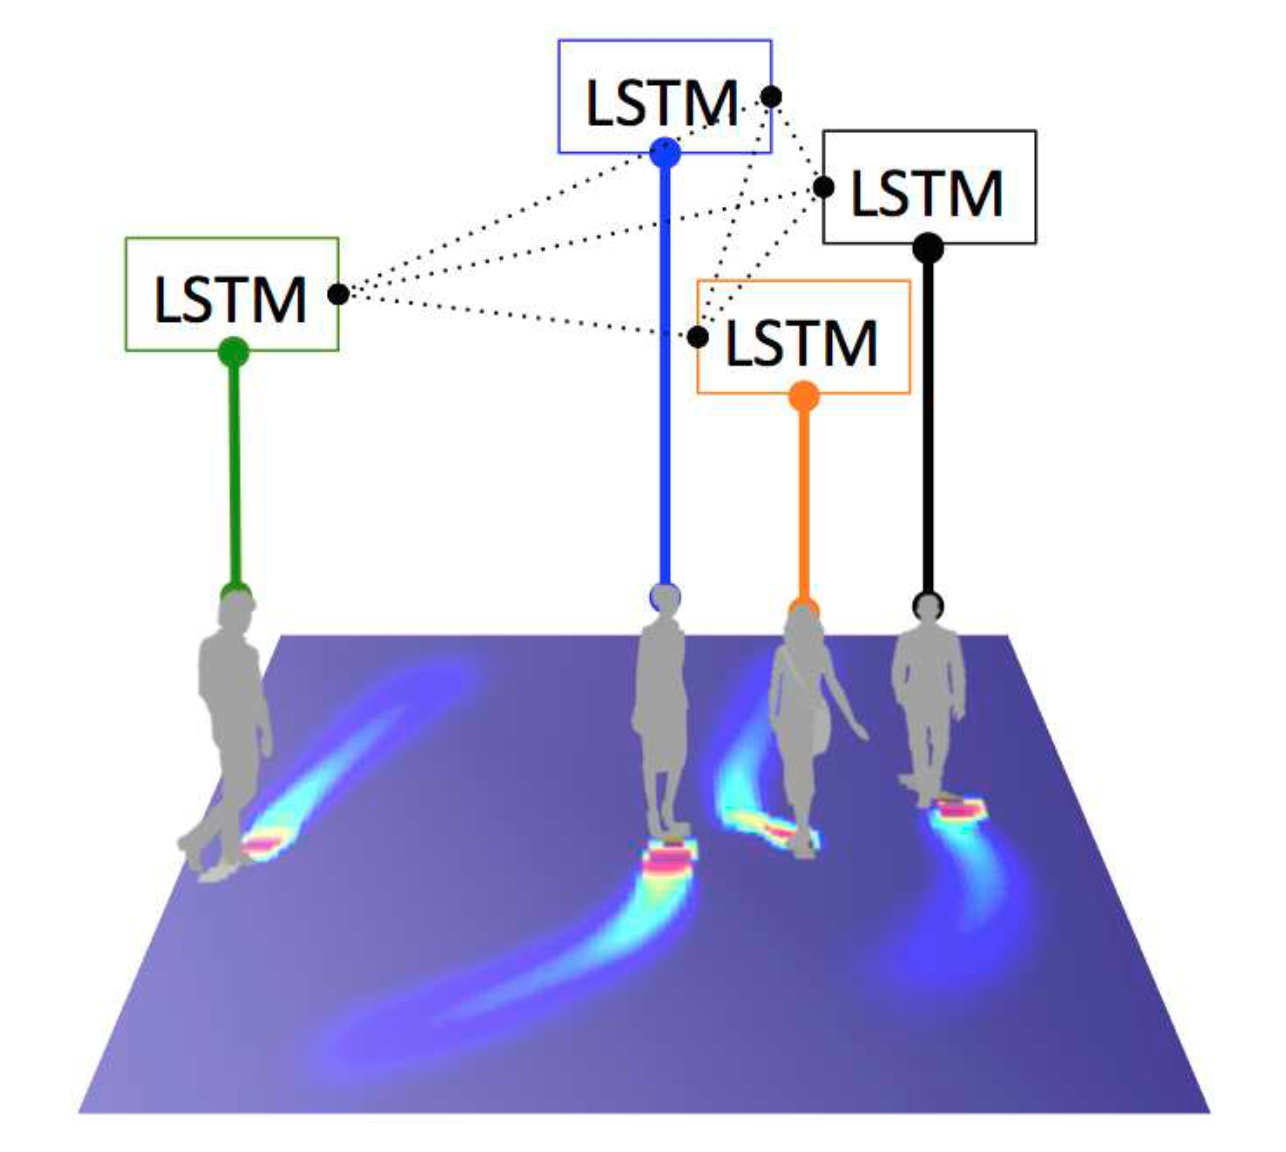
\includegraphics[scale = 0.35]{figure/socialLSTM}}
\end{minipage}
%
\section*{Idea for our Models}
\begin{minipage}[]{0.5\linewidth}
\begin{itemize}
\justifying
\item Instead of focusing on frames, prediction focus on one pedestrian
\item Special effort is put on pre-processing to make learning easier
\end{itemize}
\end{minipage}
\hfill
\begin{minipage}[]{0.5\linewidth}
\centerline {\includegraphics[scale = 0.4]{figure/OurModel}}
\end{minipage}
%----------------------------------------------------------------------------------------
%	DATA
%----------------------------------------------------------------------------------------

\section*{Pre-processing}

\textbf{Goal:} Normalize data such that every trajectory begin the same way, the model should learn more easily. \\
\vspace{1cm}

The preprocessing is divided in 5 steps:
\begin{enumerate}
\item Isolate each trajectory along with its interaction
\item Normalize the trajectories: the first point is at $(0,0)$; the second is at $(0,y_1)$
\item Calculate axis velocities $V_x$ and $V_y$
\item For each frame, if there is an interacting pedestrian we add his/her coordinates and speed otherwise we add zeros
\item Data augmentation: flip and add noise to trajectories
\end{enumerate}
\vspace{1cm}

\centerline {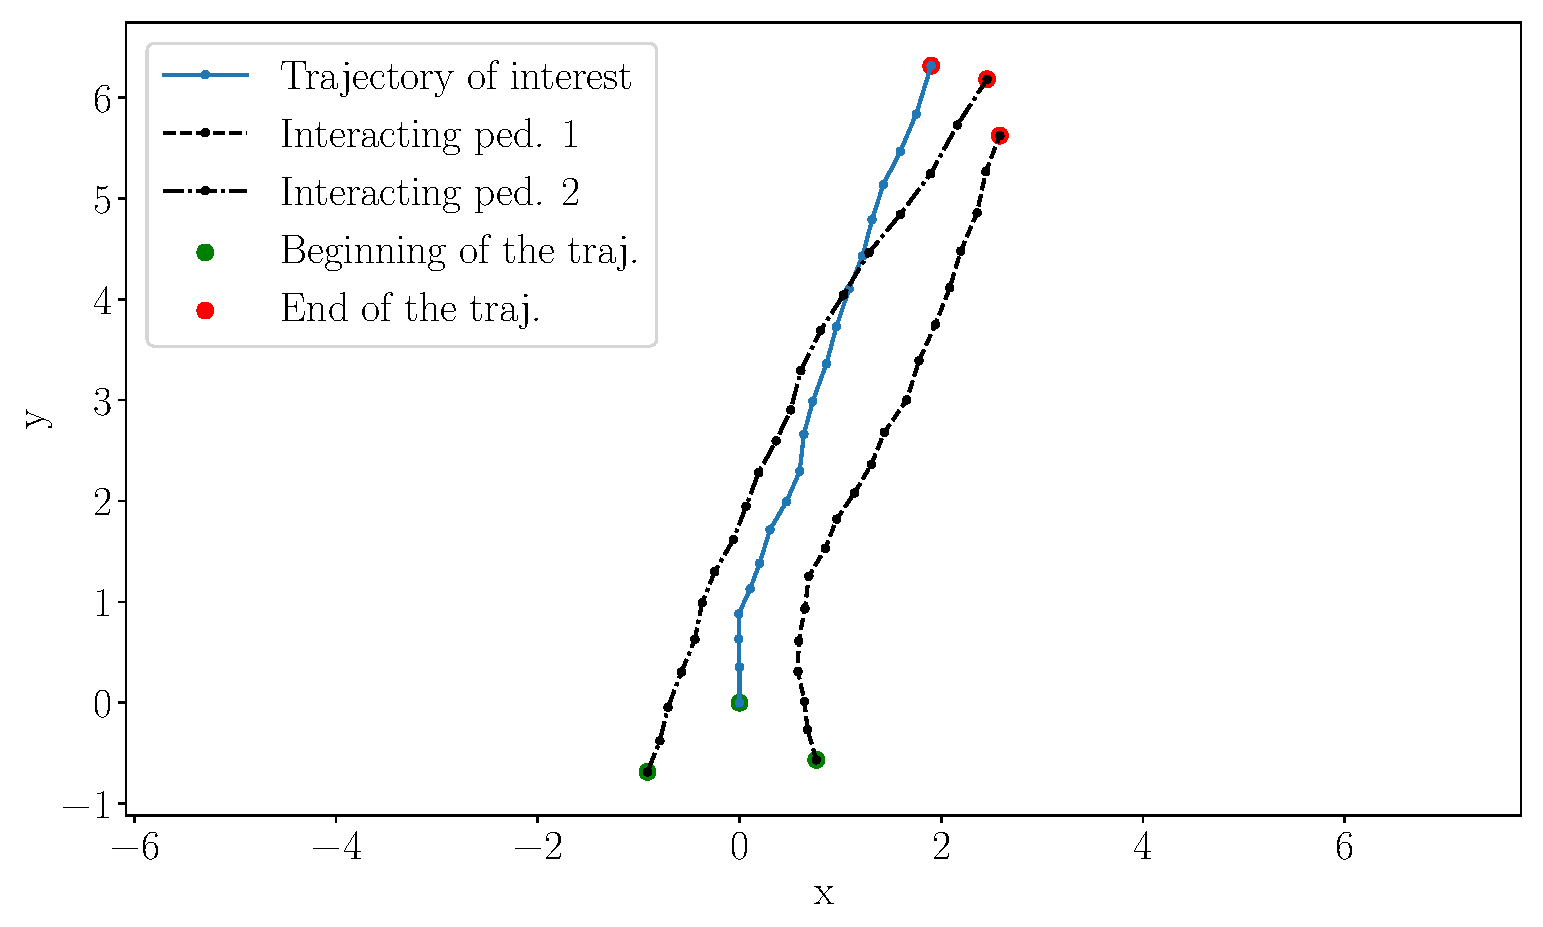
\includegraphics[width=0.2\textwidth]{figure/afterrot}}
\captionof{figure}{Example of one trajectory after pre-processing}
\vspace{3cm}
Final shape of the data:\\
\begin{minipage}[]{0.5\linewidth}
\begin{itemize}
\item Pedestrians ID
\item Frame number 
\item Twenty sets of $x$ and $y$ coordinates per pedestrian
\end{itemize}
\end{minipage}
\hfill
\begin{minipage}[]{0.5\linewidth}
\begin{tabular}{|c|c|c|c|c|c|}
\hline
Frame Number & ID & $x$ & $y$ & $ V_x$ & $V_y$ \\ \hline
        0     &  i  &  0 &  0 &  0 &  0 \\ \hline
        10     &  i  &  0 &  $y_1$ &  0 &  $V_{y_1}$ \\ \hline
        \vdots     &  \vdots &  \vdots & \vdots &  \vdots &  \vdots \\ \hline
\end{tabular}
\end{minipage}
%------------------------------------------------

\section*{Objectives}

\begin{itemize}
\item Train on the 10 first coordinates and speed and their interaction
\item Predict the next 10 
\item Inputs have the following shape: $[10,N,4 * N_{inter}]$ 
\end{itemize}

\centerline {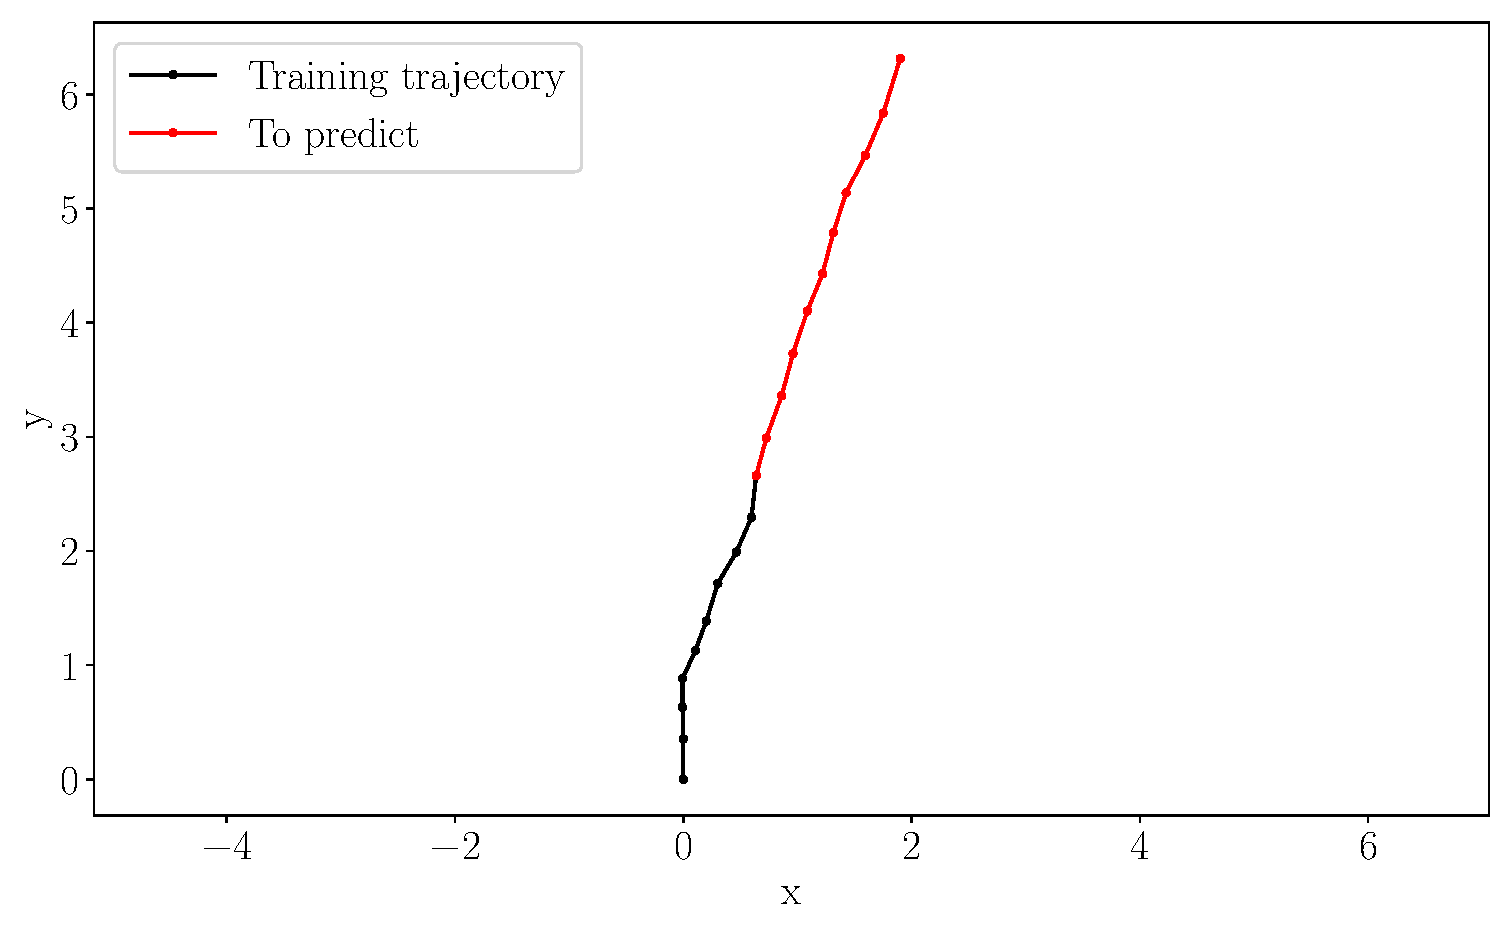
\includegraphics[width=0.2\textwidth]{figure/examplepres}}

%----------------------------------------------------------------------------------------
%	Models 
%----------------------------------------------------------------------------------------

\section*{Models}
\textbf{Inputs:} sequence of coordinates and velocities of the trajectory of interest and of the interacting trajectories\\
\textbf{Outputs:} sequence of predicted coordinates and velocities for the trajectory of interest.\\

\vspace{1.5cm}

\begin{minipage}[]{0.5\linewidth}
\subsection*{CNN}
\centerline {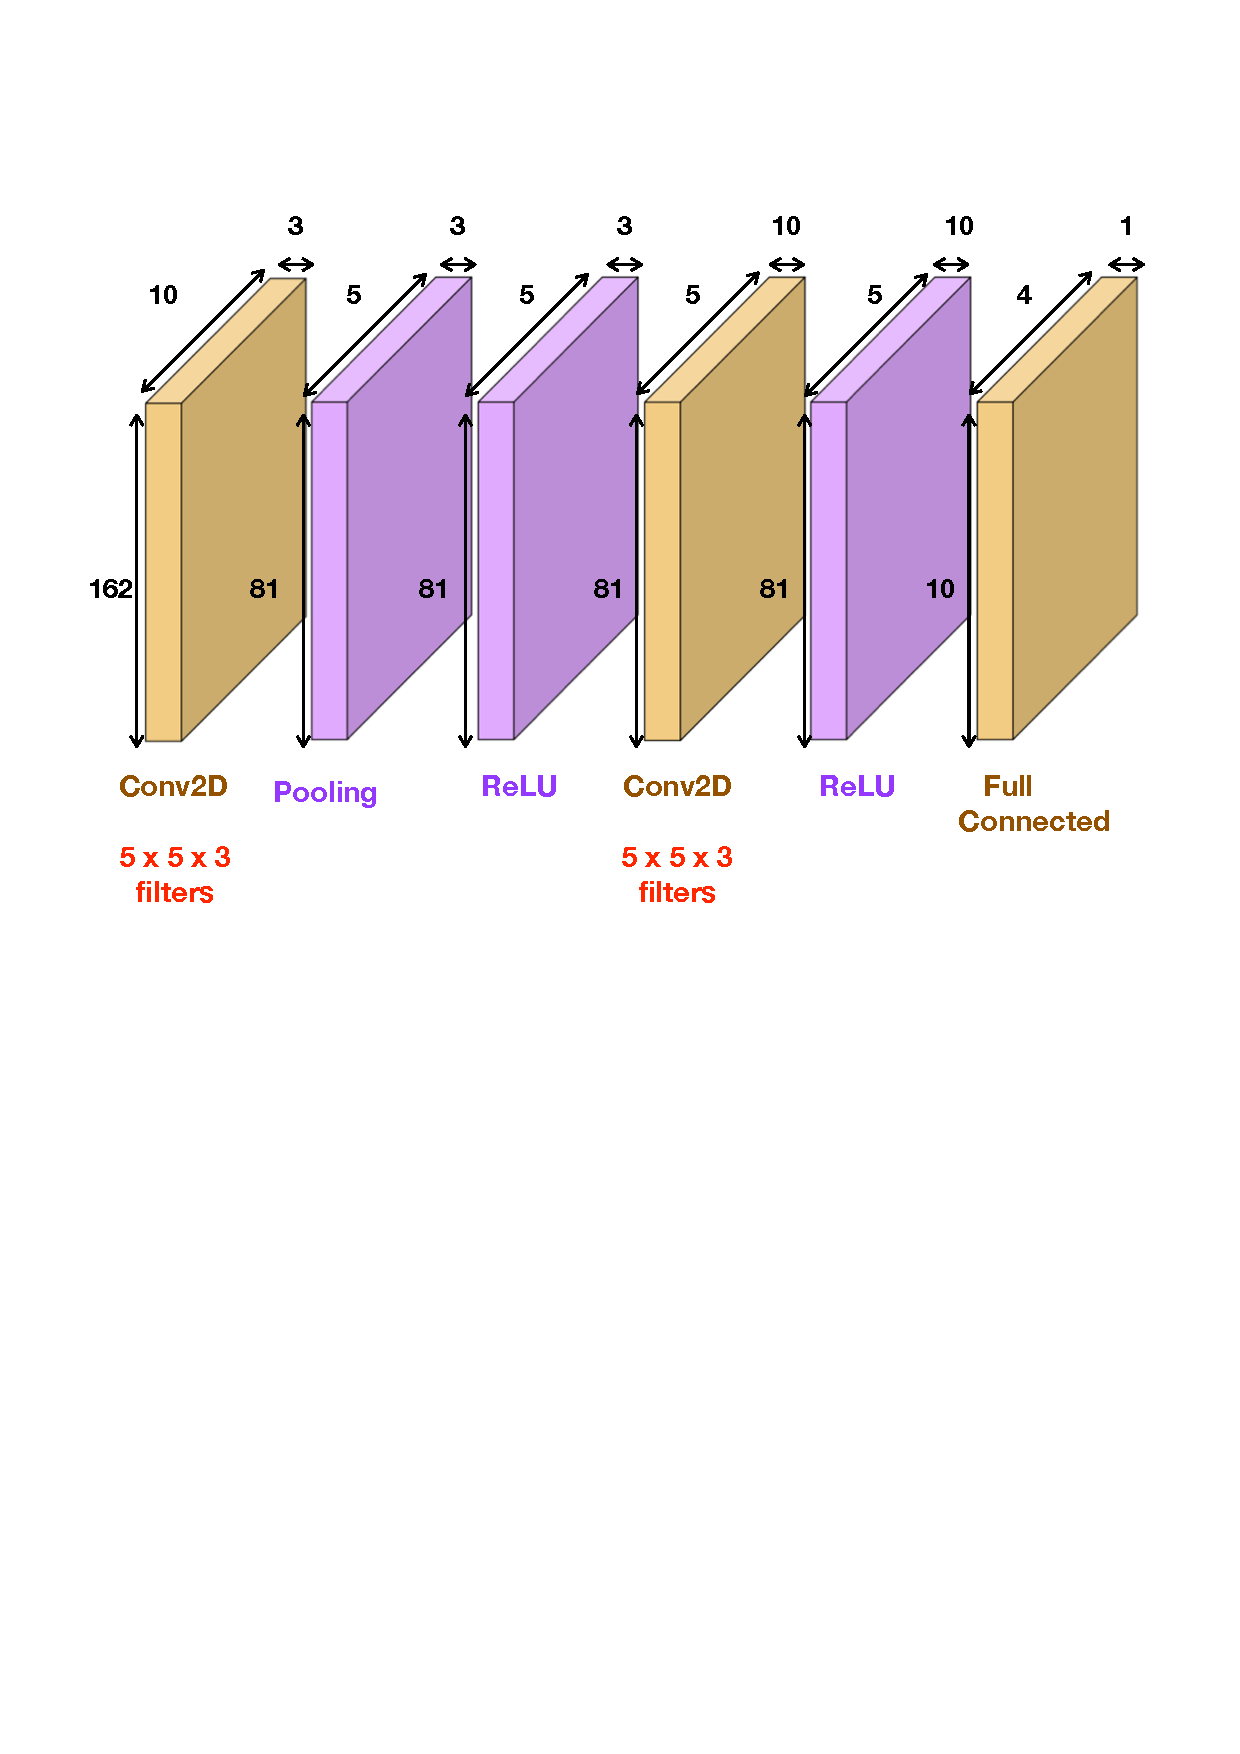
\includegraphics[width=0.6\textwidth]{figure/CNN}}
\vspace{3cm}
\end{minipage}
\hfill
\begin{minipage}[]{0.5\linewidth}
\subsection*{LSTM}

\centerline {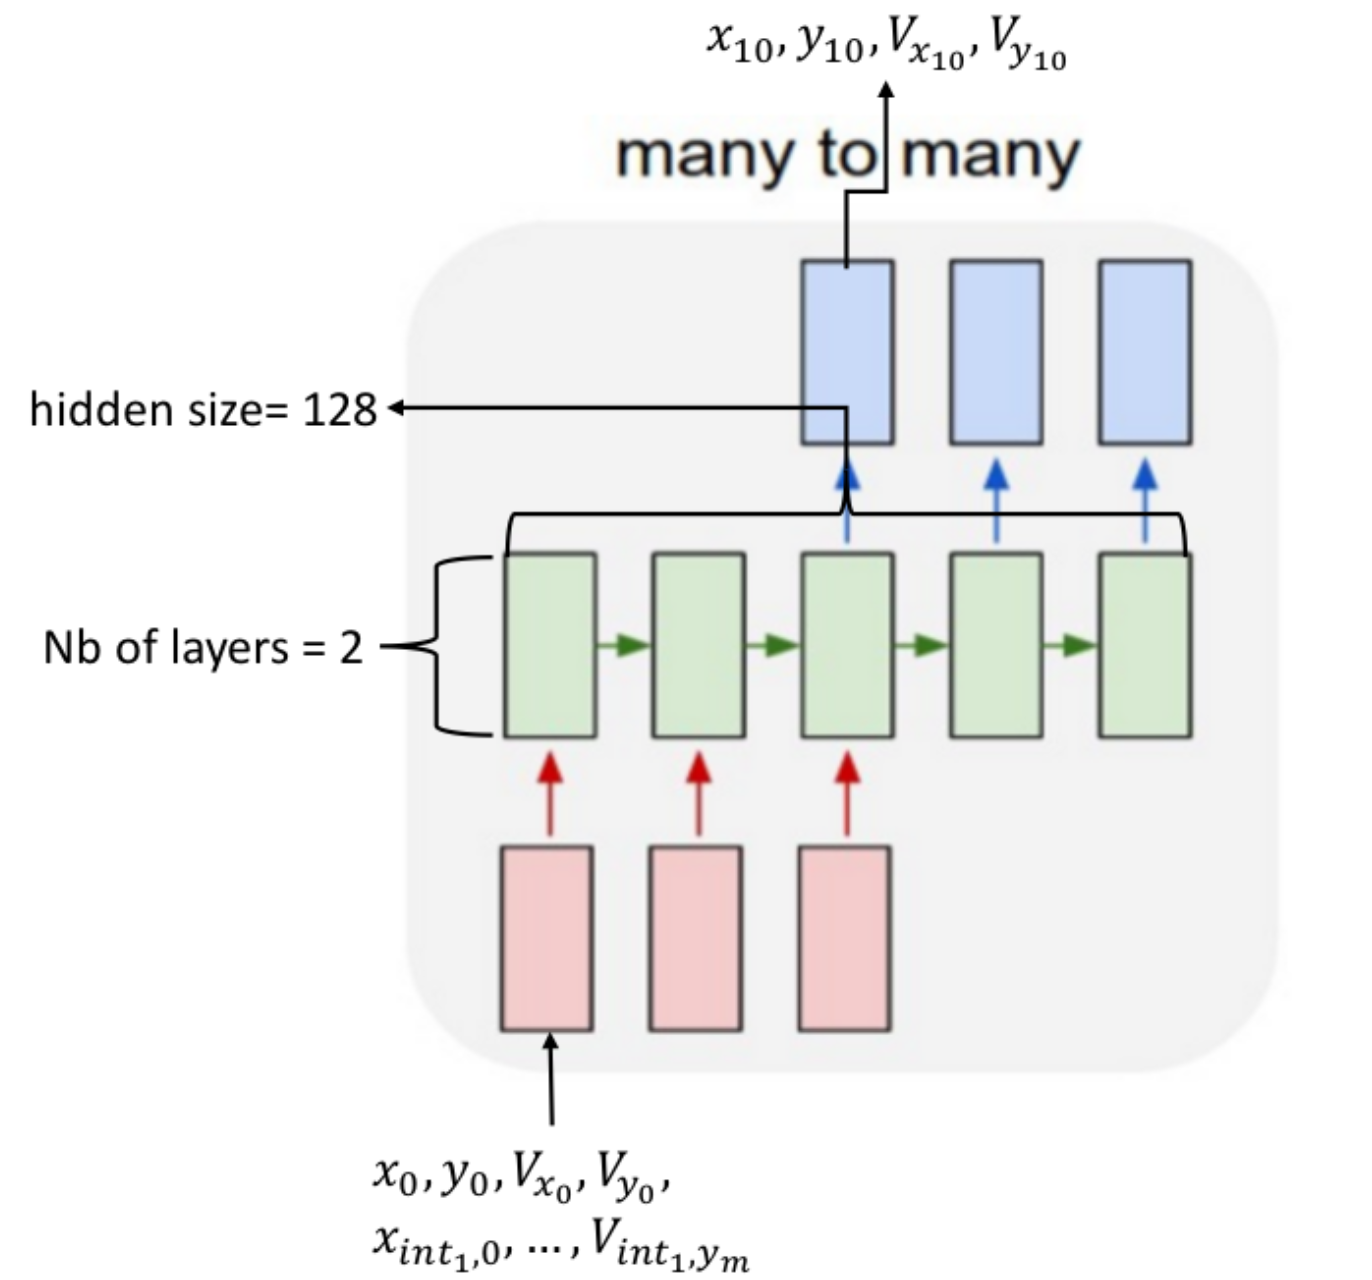
\includegraphics[width=0.6\textwidth]{figure/manytomany}}
\end{minipage}

%----------------------------------------------------------------------------------------
%	Results
%----------------------------------------------------------------------------------------

\section*{Results}
\subsection*{Precision indicators}
To calculate the correctness of the prediction two indicators are used:
\begin{enumerate}
\justifying
\item The final displacement error: $e_{fin} = \sqrt{(X_{gt,n}-X_{pred,n})^2}$
\item The mean displacement error: $e_{mean} = \sqrt{\frac{\sum_{i=0}^n(X_{gt,i}-X_{pred,i})^2}{(n)}}$
\end{enumerate}
\vspace{0.5cm}

\subsection*{Post-processing}
Depending on the inputs two ways are possible to find the predicted coordinates:
\begin{enumerate}
\justifying
\item If the coordinates are predicted: directly use them
\item If the velocities are predicted: $X_{t} = X_{t-1} + V_{t}\cdot 0.4$, with $0.4$ the time between two frames in seconds
\end{enumerate}

\subsection*{Model tests case}
Four different cases, that corresponds to four losses, are tested for each model:
\begin{enumerate}
\justifying
\item Predict coordinates with loss defines as $L_1 = (X-X_{pred})^2$ with $X = [x,y]$
\item Predict speeds with loss defines as $L_2 = (V-V_{pred})^2$ with $V = [V_x,V_y]$ 
\item Predict both coordinates and speeds with loss defines as $L = L_1 + L_2$
\item Predict both coordinates and speeds with loss defines as $L = L_1 + L_2 + L_3 $, with $L_3 = (X- X_{t-1} + V_t*0.4)^2$
\end{enumerate}
\vspace{0.5cm}
\begin{minipage}[]{0.5\linewidth}
\subsection*{Trajectory type}
\begin{enumerate}
\justifying
\item Static
\item Linear trajectories
\item Non-linear trajectories
\end{enumerate}
\end{minipage}
\hfill
\begin{minipage}[]{0.5\linewidth}
\subsection*{Linear prediction results}
\begin{itemize}
\item Type 1: \emph{Mean} = 0.141, \emph{Final} = 0.322
\item Type 2: \emph{Mean} = 0.541, \emph{Final} = 0.93
\item Type 3: \emph{Mean} = 0.651, \emph{Final} = 1.457
\item Total: \emph{Mean} = 0.512, \emph{Final} = 0.982 
\end{itemize}
\end{minipage}

\vspace{0.5cm}

\subsection*{Models results}
\begin{center}
\begin{tabular}{cc|c|c|c|c|c|c|c|c|}
\cline{3-10}
\multicolumn{1}{l}{}                                     &                & \multicolumn{4}{c|}{\textbf{CNN}}                                    & \multicolumn{4}{c|}{\textbf{LSTM}}                                                          \\ \cline{3-10} 
                                                         &                & \textbf{Type 1} & \textbf{Type 2} & \textbf{Type 3} & \textbf{Total} & \textbf{Type 1} & \textbf{Type 2} & \textbf{Type 3} & \textbf{Total}                        \\ \hline
\multicolumn{1}{|c|}{}                                   & \textbf{Mean}  &4.696                 & 5.144                &4.674                 &4.176                & 1.309            & 0.777           & 0.862           & 0.877                                 \\ \cline{2-10} 
\multicolumn{1}{|c|}{\multirow{-2}{*}{\textbf{Coord.}}} & \textbf{Final} &10.246                 & 7.009                &10.501                 &5.602                & 1.385           & 0.92           & 1.108           & 1.037                                \\ \hline
\multicolumn{1}{|c|}{}                                   & \textbf{Mean}  &0.567                 &5.133                 &1.911                 &4.17                & 0.726           & 0.573           & 0.651           & 0.616 \\ \cline{2-10} 
\multicolumn{1}{|c|}{\multirow{-2}{*}{\textbf{Speed}}} & \textbf{Final} &0.77                 &6.971                 &3.882                 &5.587                & 1.412           & 1.045           & 1.231           & 1.148 \\ \hline
\multicolumn{1}{|c|}{}                                   & \textbf{Mean}  &1.269      &5.134                 &1.762                 &{\color[HTML]{FE0000} \textbf{4.163}}                & 0.695           & 0.532           & 0.627           &  {\color[HTML]{FE0000} \textbf{0.581}}                                 \\ \cline{2-10} 
\multicolumn{1}{|c|}{\multirow{-2}{*}{\textbf{2 Losses}}} & \textbf{Final} &2.727                 &6.978                 &3.546                 &{\color[HTML]{FE0000} \textbf{5.57}}                & 1.302           & 0.963           & 1.2           &  {\color[HTML]{FE0000} \textbf{1.076}}                                 \\ \hline
\multicolumn{1}{|c|}{}                                   & \textbf{Mean}  &0.549                 &5.135                 &3.829                 &4.163                & 0.748           & 0.607           & 0.681           & 0.647                                  \\ \cline{2-10} 
\multicolumn{1}{|c|}{\multirow{-2}{*}{\textbf{3 Losses}}} & \textbf{Final} &0.758                 &6.983                 &4.962                 &5.573                & 1.364           & 1.072            & 1.308           & 1.177                                  \\ \hline
\end{tabular}
\end{center}
\subsection*{Observation}
\begin{itemize}
\justifying
\item Best results are the same for both models: case with two losses, one for coordinates and the other for velocities
\item LSTM has much better results than CNN: memory capacities of the cells is useful in sequence to sequence prediction
\item Three losses model might be too complicated for learning
\item Good results for type 2 and 3 trajectories but struggle for type 1
\item Global results is better with linear prediction, but without type 1 LSTM is better
\end{itemize}

\section*{Representation}

\begin{minipage}[]{0.5\linewidth}
Non linear trajectory with good prediction:\\
\centerline {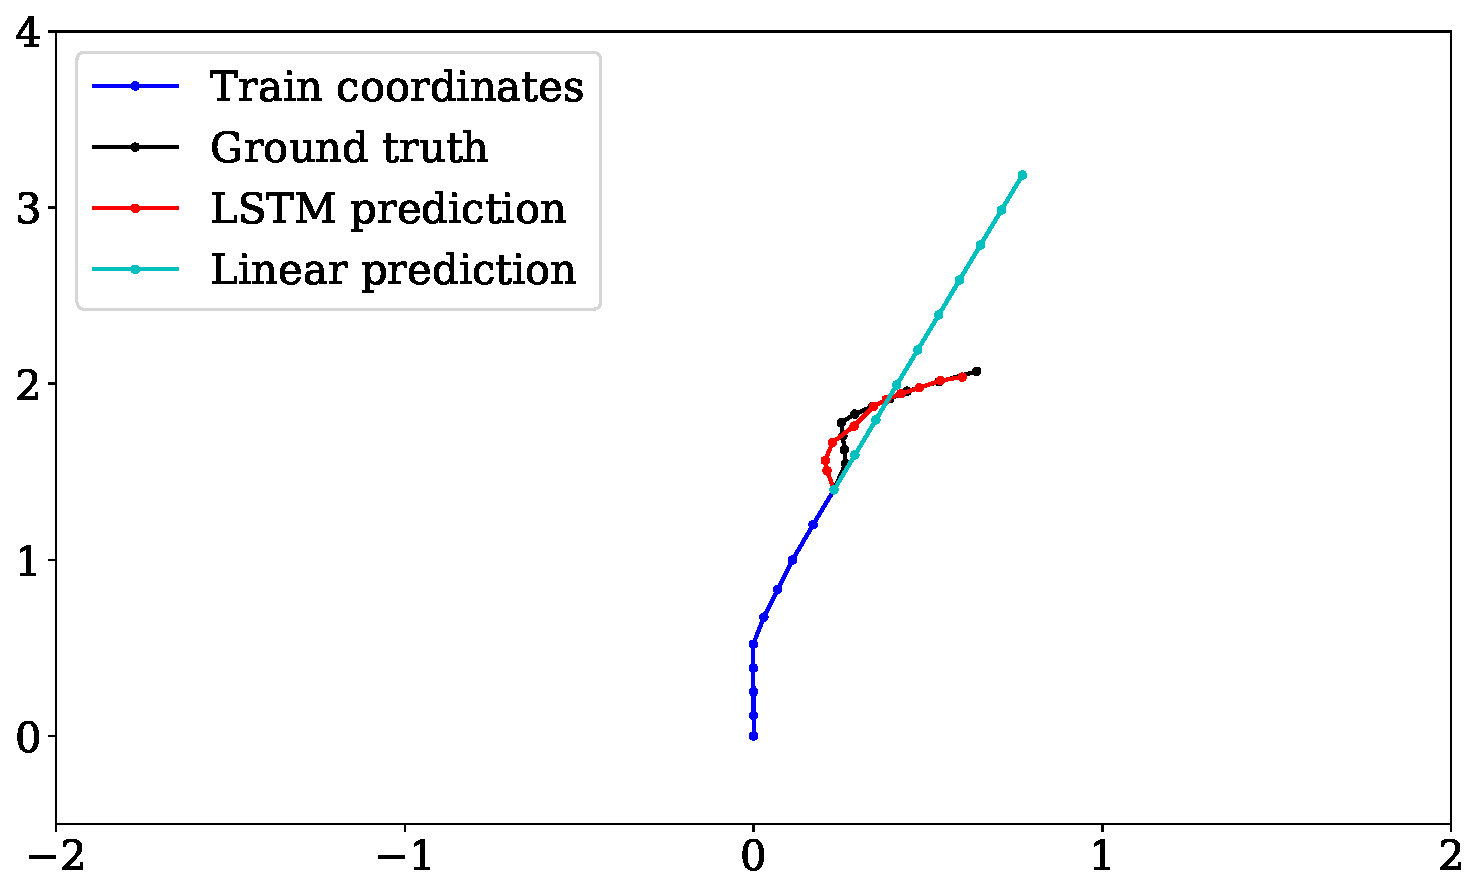
\includegraphics[width=0.8\textwidth]{figure/fig_1552}}
\end{minipage}
\hfill
\begin{minipage}[]{0.5\linewidth}
Non linear trajectory with bad prediction:\\
\centerline {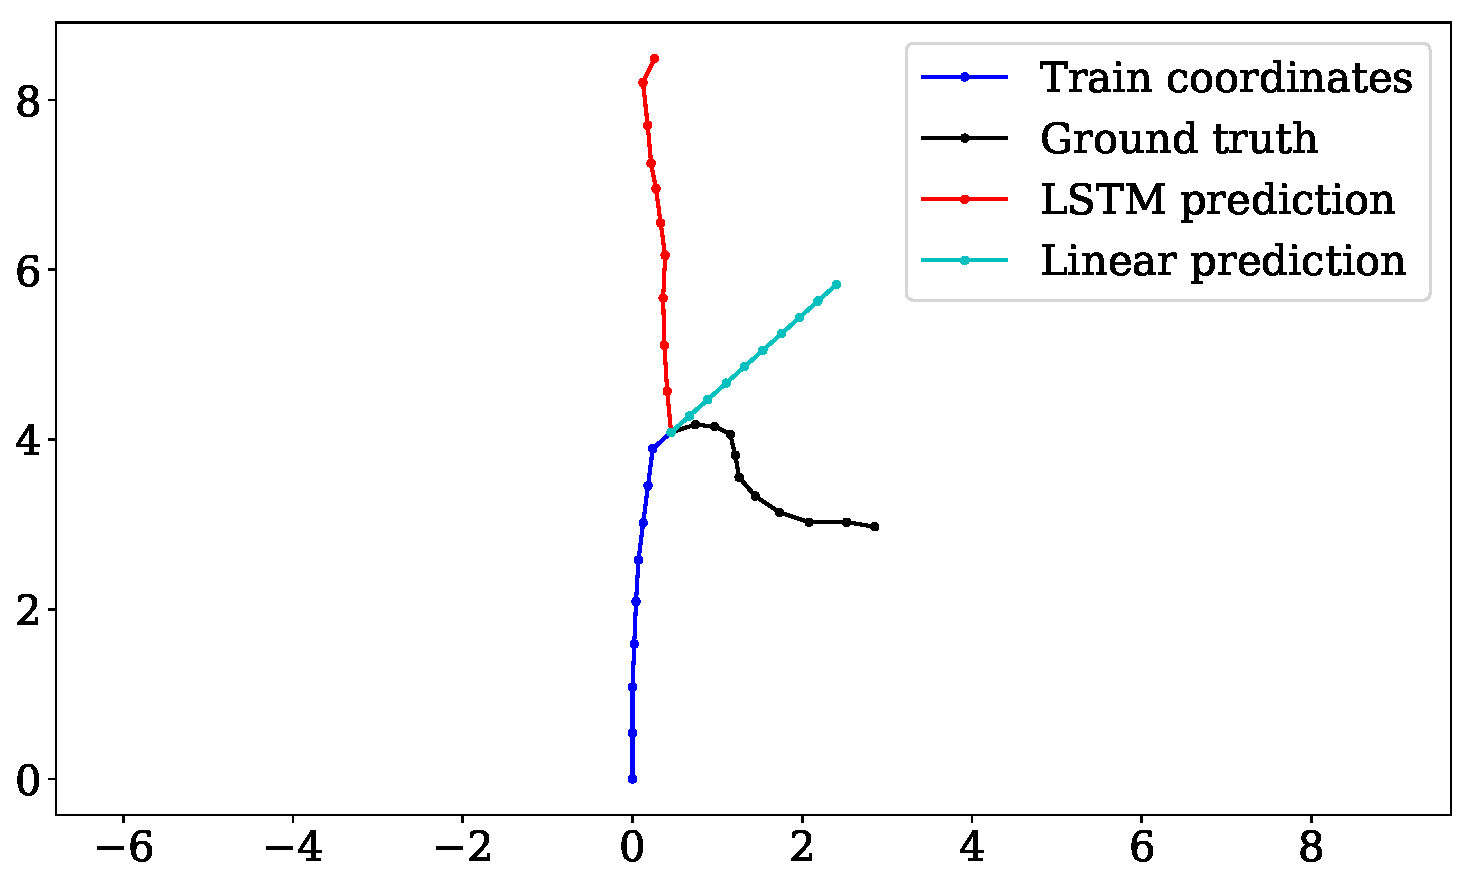
\includegraphics[width=0.8\textwidth]{figure/fig_1621}}
\end{minipage}

%----------------------------------------------------------------------------------------
%	FORTHCOMING RESEARCH
%----------------------------------------------------------------------------------------

\section*{Issues \& Future work}

Vivamus molestie, risus tempor vehicula mattis, libero arcu volutpat purus, sed blandit sem nibh eget turpis.

 %----------------------------------------------------------------------------------------
%	REFERENCES
%----------------------------------------------------------------------------------------

\nocite{*} % Print all references regardless of whether they were cited in the poster or not
\bibliographystyle{plain} % Plain referencing style
\bibliography{sample} % Use the example bibliography file sample.bib


\end{multicols}
\end{document}